% ==============================================================================
\section{Motivation \& Background}
% ------------------------------------------------------------------------------
\begin{frame}{Research Question}
  \paragraph{Research Question}
  Impact of \textbf{hotspot} vs \textbf{non-hotspot}
  \covid vaccine prioritization in Ontario
  \bigskip
  \paragraph{Transmission Model}
  \begin{itemize}
    \item 513 FSA (first 3 postal code digits) $\rightarrow$ \textbf{10 deciles} by cumulative cases
    \item \textbf{12 age} groups: [0-11, 12-15, 16-39, 40-44, \dots, 75-79, 80+]
    \item \textbf{4* contact types}: household, school, work, other
    \item \covid stuff \dots
  \end{itemize}
\end{frame}
% ------------------------------------------------------------------------------
\begin{frame}{Ontario FSA, stratified by deciles of cumulative \covid incidence}
  \begin{minipage}{0.30\linewidth}
    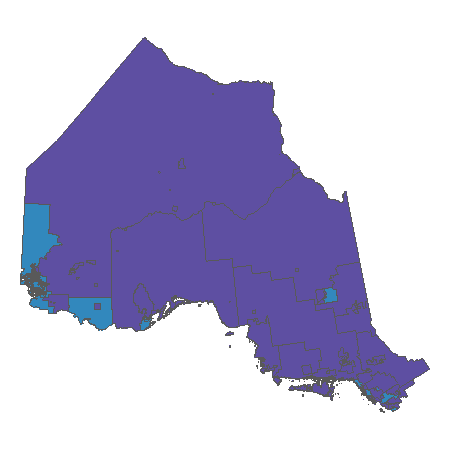
\includegraphics[width=\linewidth]{ontario-north}
  \end{minipage}%
  \begin{minipage}{0.35\linewidth}
    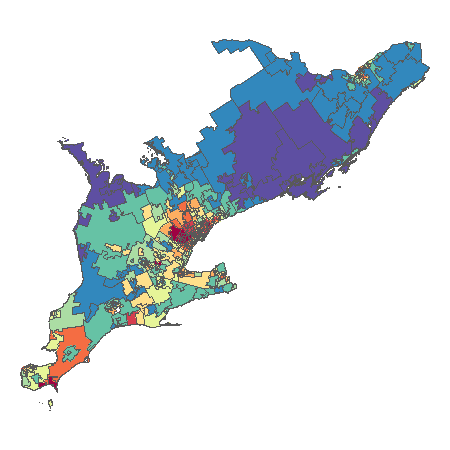
\includegraphics[width=\linewidth]{ontario-south}
  \end{minipage}%
  \begin{minipage}{0.35\linewidth}
    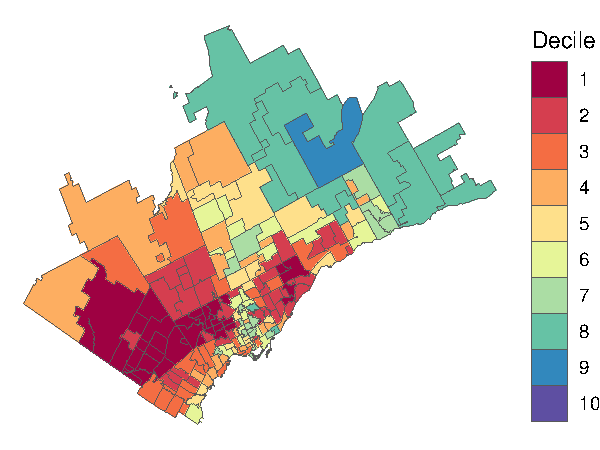
\includegraphics[width=\linewidth]{ontario-gta}
  \end{minipage}%
\end{frame}
% ------------------------------------------------------------------------------
\begin{frame}{\Covid incidence by deciles (FSA): consistent differences}
  \centering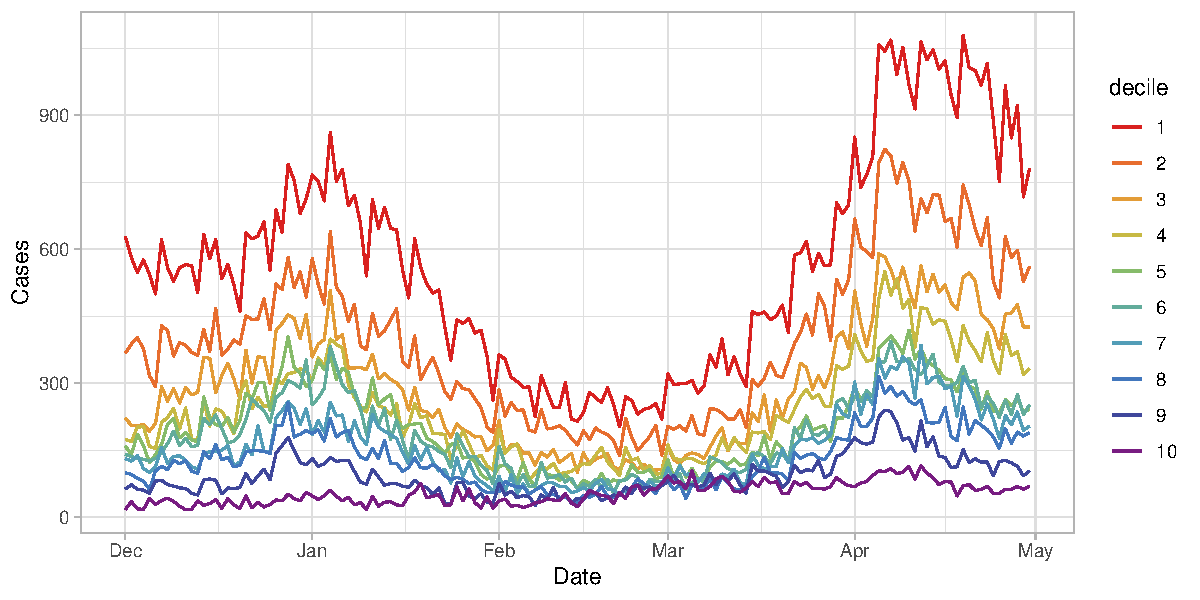
\includegraphics[height=\maxheight]{Yg}
\end{frame}
% ------------------------------------------------------------------------------
\begin{frame}{Objective}
  Develop a \textbf{mixing matrix} (\# contacts formed \& with whom) stratified by:
  \bigpar
  \begin{minipage}{.33\linewidth}
    \begin{itemize}
      \item self decile, $g$
      \item self age, $a$
    \end{itemize}
  \end{minipage}%
  \begin{minipage}{.33\linewidth}
    \begin{itemize}
      \item other decile, $g'$
      \item other age, $a'$
    \end{itemize}
  \end{minipage}%
  \begin{minipage}{.33\linewidth}
    \begin{itemize}
      \item contact type, $y$
      \item calendar month, $t$
    \end{itemize}
  \end{minipage}
  \bigpar
  Dimensions: $10 \times 12 \times 10 \times 12 \times 4 \times t$
\end{frame}
% ------------------------------------------------------------------------------
\begin{frame}{Methods Overview}
  \begin{enumerate}
    \item Mobility Patterns: $gg't$
    \item Age Mixing: $aa'y$
    \item Integrated Age \& Mobility Mixing: $gag'a'yt$
  \end{enumerate}
\end{frame}
% ==============================================================================
\section{Mobility Matrix}
% ------------------------------------------------------------------------------
\begin{frame}{Mobility Data}
  \begin{minipage}{0.55\textwidth}
    \ttilde 2\,\% Ontario devices, Jan--Dec 2020
    \medpar
    Define:
    \begin{itemize}
      \item \textbf{Household}: \ttilde 150m\tss{2} tile with\\
      most evening time per month
      \item \textbf{Home FSA}: FSA $n$ containing Household
      \item \textbf{Visited FSA}: 2+ hours in another FSA $n'$
      \item \textbf{Away Time:} \% time outside Household\\
      stratified by Home vs Visited FSA
    \end{itemize}
    \medpar
    Repeat for each month $t$
  \end{minipage}%
  \begin{minipage}{0.45\textwidth}
    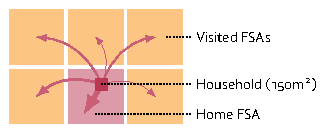
\includegraphics[width=\linewidth]{t-away}
  \end{minipage}
\end{frame}
% ------------------------------------------------------------------------------
\begin{frame}{Mobility Metrics, by FSA $n$ and Month $t$}
  \bigpar
  \begin{tabular}{ll}
    \textbf{Inter-FSA Mobility}, conditional probability of destination $n'$: &
    $\displaystyle B^c_{nn't} = \frac{V_{nn't}}{\sum_{n'}V_{nn't}}$
    \\[\eqtabsep]
    \textbf{Relative Time Away} (TA) from home, vs reference $t_0$: &
    $\displaystyle\rho_{nt} = \frac{{TA}_{nt}}{{TA}_{nt_0}}$
    \\[\eqtabsep]
    \textbf{Proportion Time Away in Home FSA} of total Time Away: &
    $\displaystyle\phi_{nt} = \frac{{TA}^{(h)}_{nt}}{{TA}_{nt}}$
    \\[\eqtabsep]
  \end{tabular}
  \bigpar
  Later: aggregate from FSA $n$ $\rightarrow$ decile $g$
\end{frame}
% ------------------------------------------------------------------------------
\begin{frame}{Mobility Metrics: Inter-FSA Mobility}
  \centering
  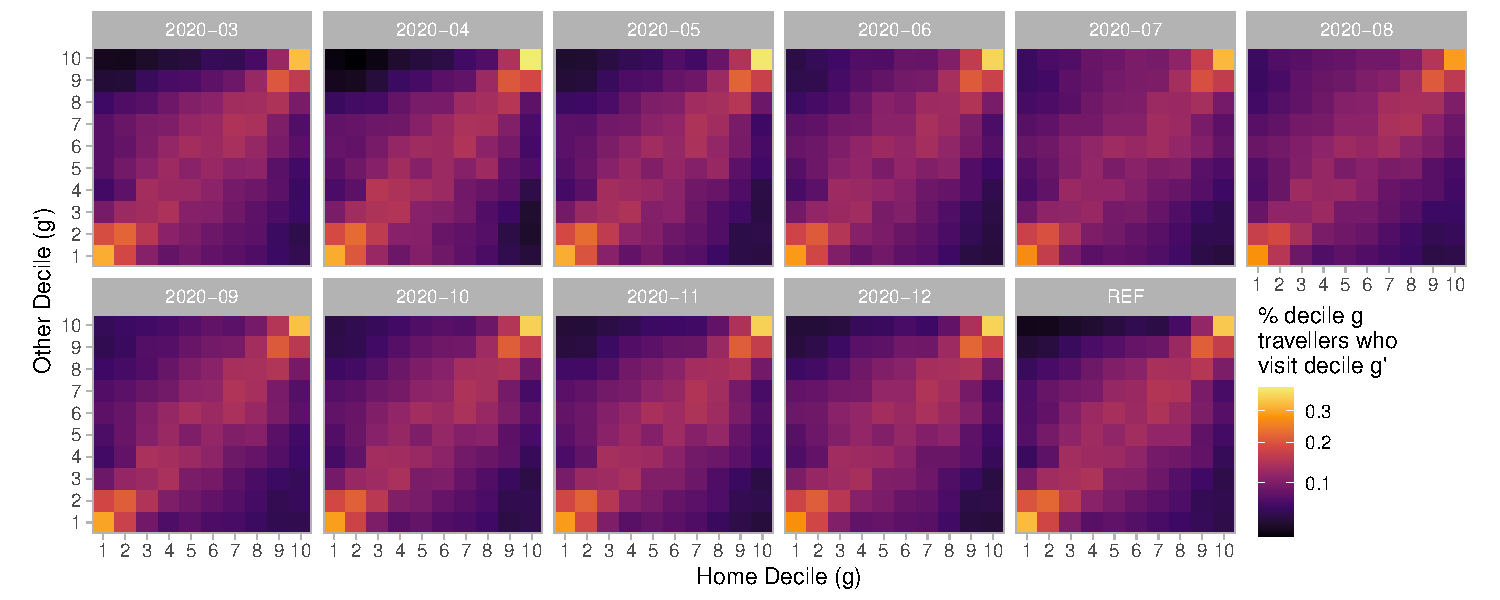
\includegraphics[width=\linewidth]{Bcggt}
\end{frame}
% ------------------------------------------------------------------------------
\begin{frame}{Mobility Metrics: Time Away}
  \centering
  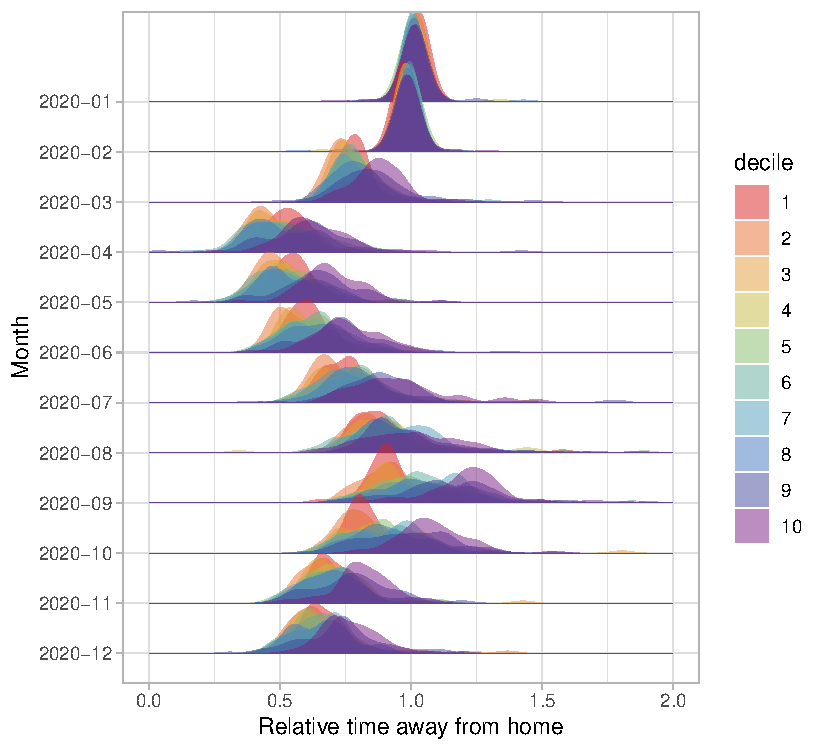
\includegraphics[height=\maxheight]{rho-gnt}
  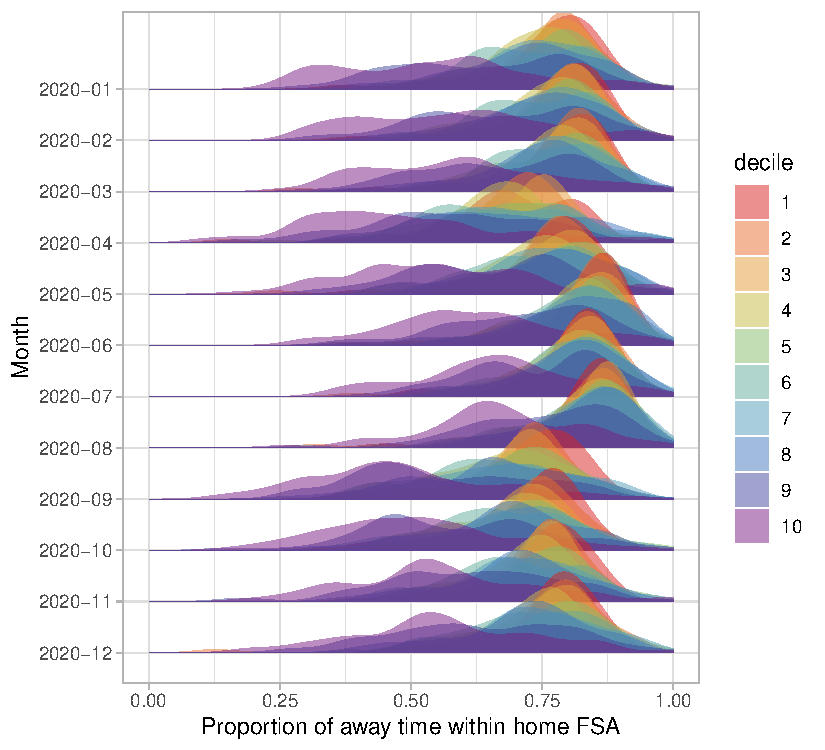
\includegraphics[height=\maxheight]{phi-gnt}
\end{frame}
% ------------------------------------------------------------------------------
\begin{frame}{Mobility Matrix: Equation}
  \begin{equation*}
    B_{gg't} = 
      \ulabel{\rho_{gt}}{overall mobility\quad\quad} \Big[
      \ulabel{(\phi_{gt})\,\delta_{gg'}}{\quad\quad intra-decile} +
      \ulabel{(1-\phi_{gt}\,B^c_{gg't})}{inter-decile}
    \Big]
  \end{equation*}
\end{frame}
% ------------------------------------------------------------------------------
\begin{frame}{Does inter-FSA mobility $B^c_{gg'}$ change by month?}
  \only<1>{\centering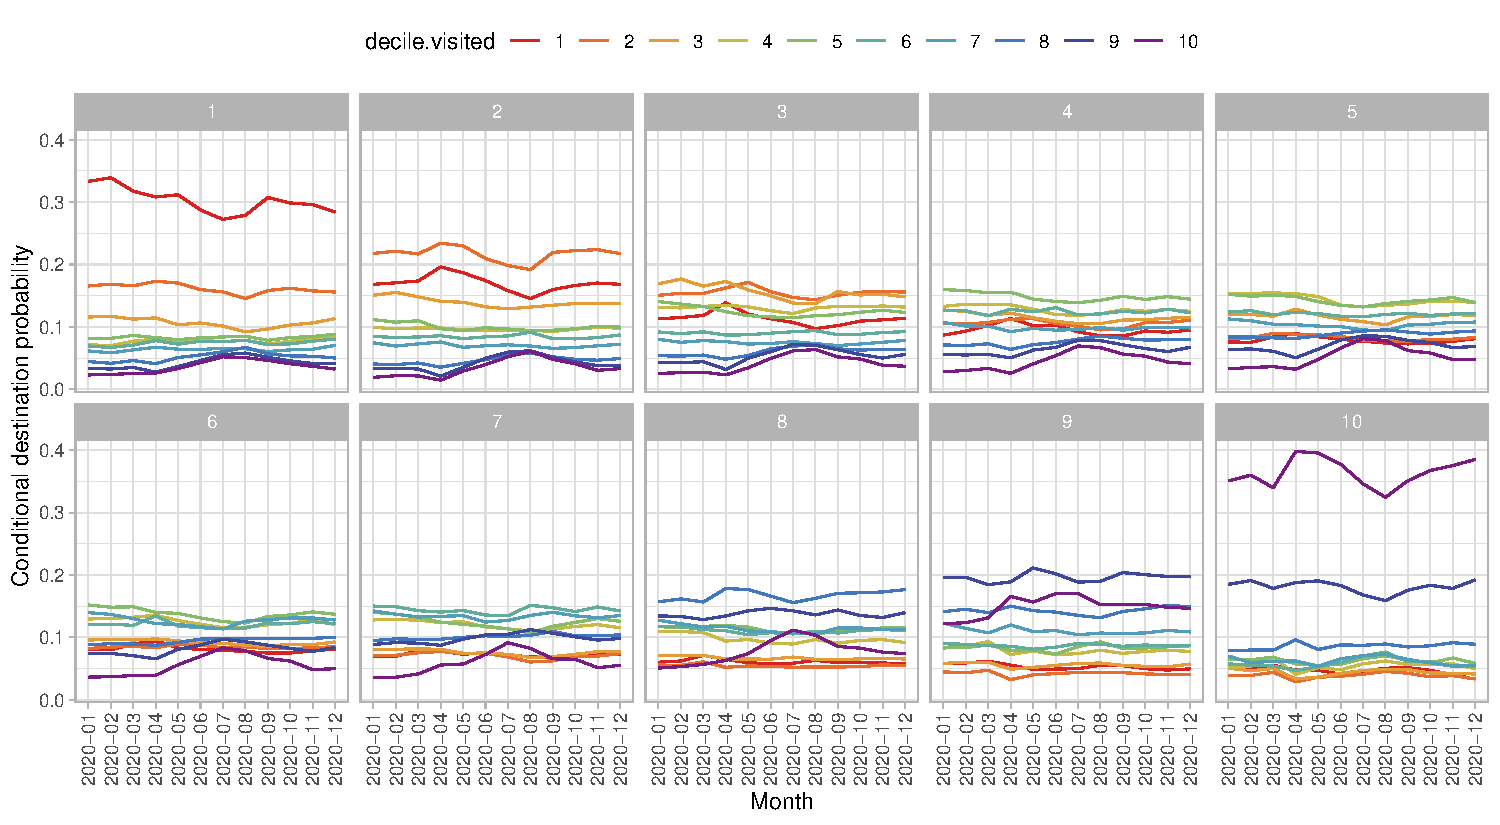
\includegraphics[height=\maxheight]{Bc-gt}}%
  \only<2>{\centering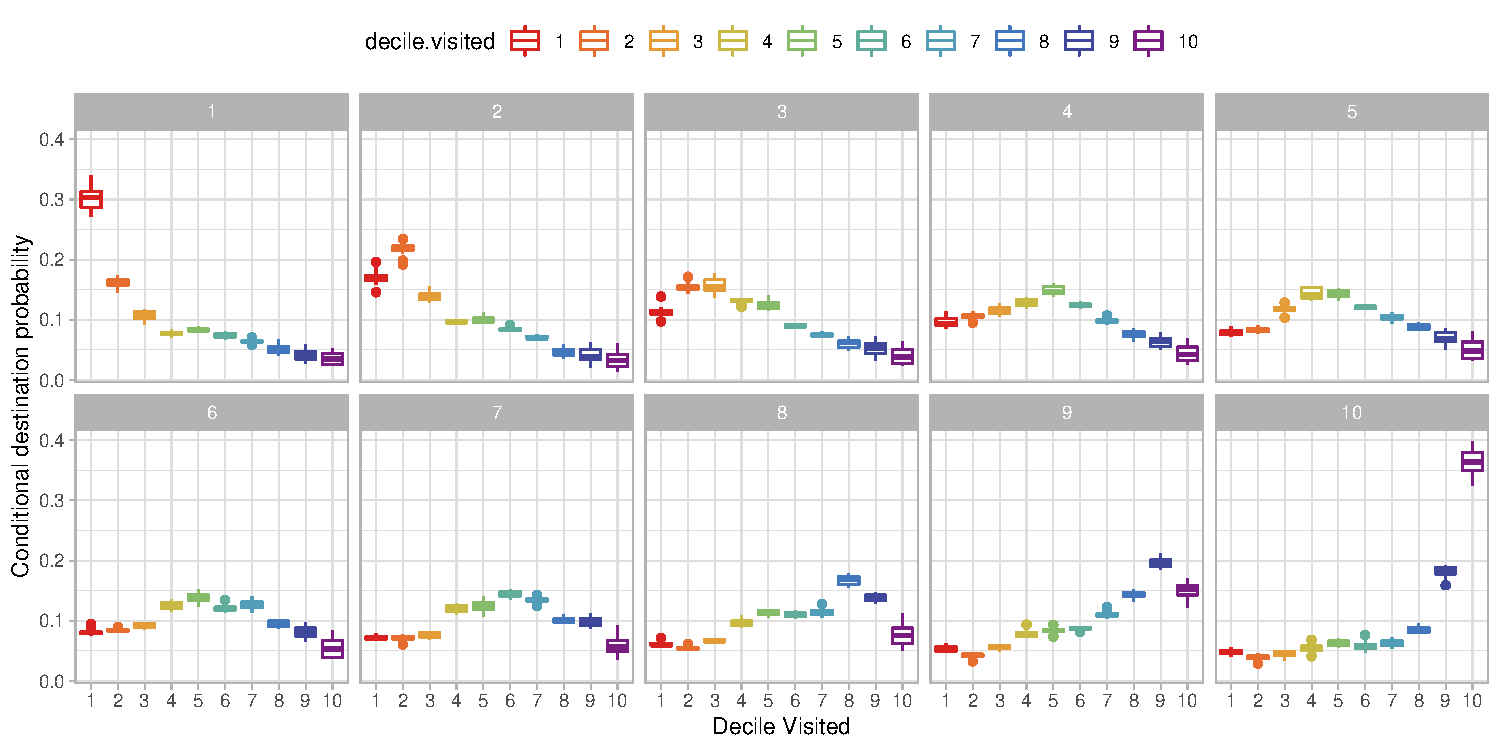
\includegraphics[height=\maxheight]{Bc-box}}
\end{frame}
% ------------------------------------------------------------------------------
\begin{frame}{Does overall time away per decile $\rho_g$ change by month?}
  \centering
  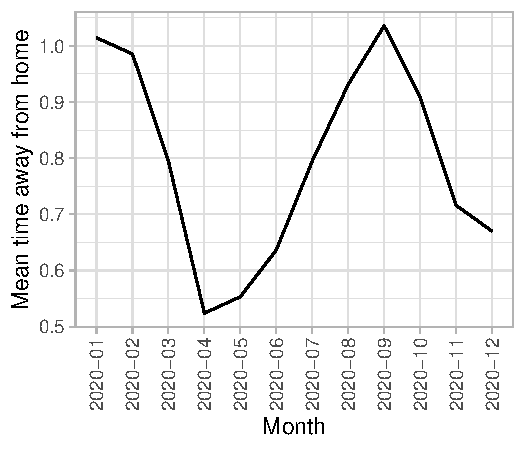
\includegraphics[width=0.297\linewidth]{rho-t}%
  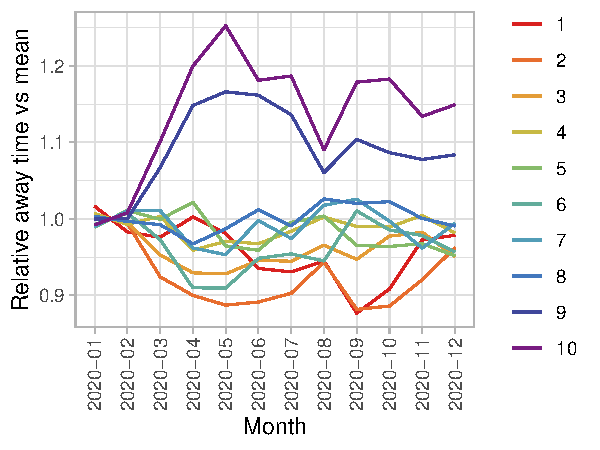
\includegraphics[width=0.333\linewidth]{R-rho-gt}%
  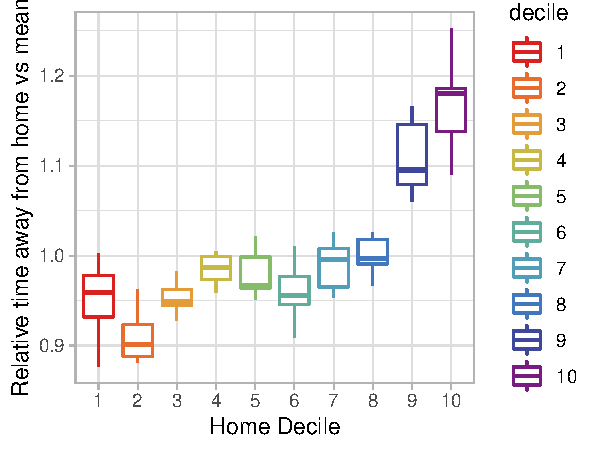
\includegraphics[width=0.333\linewidth]{R-rho-box}
\end{frame}
% ------------------------------------------------------------------------------
\begin{frame}{Does \% time away within home FSA per decile $\phi_g$ change by month?}
  \centering
  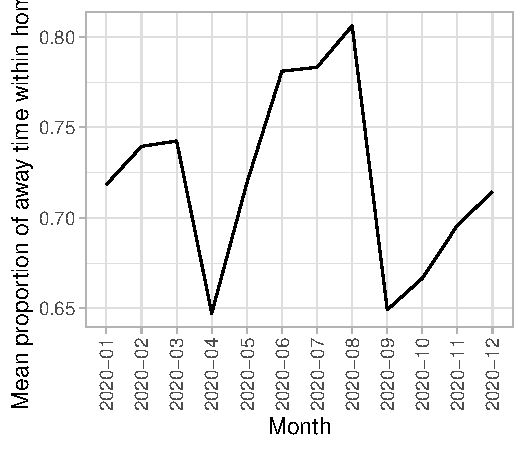
\includegraphics[width=0.297\linewidth]{phi-t}%
  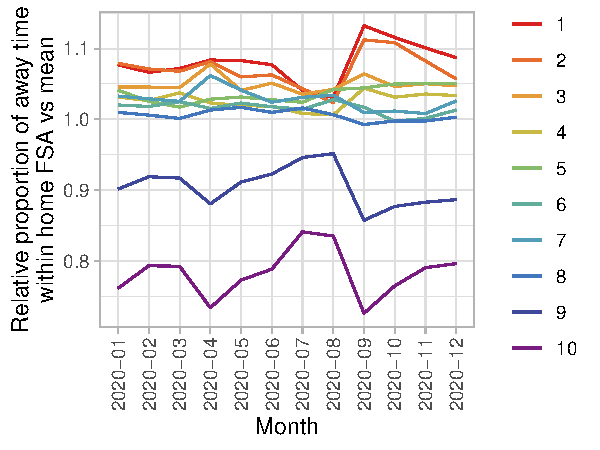
\includegraphics[width=0.333\linewidth]{R-phi-gt}%
  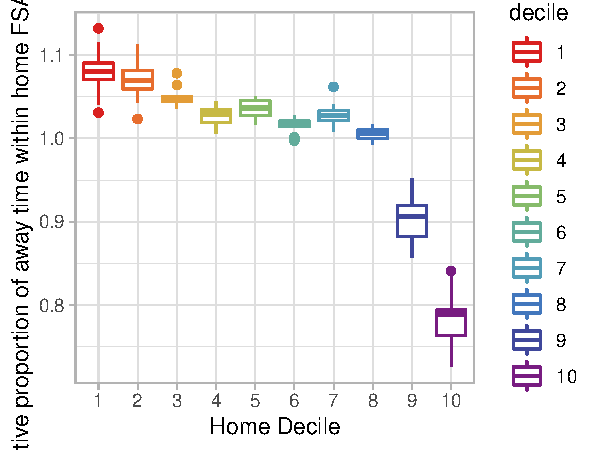
\includegraphics[width=0.333\linewidth]{R-phi-box}
\end{frame}
% ------------------------------------------------------------------------------
\begin{frame}{Mobility Matrix: Equation with 1 (or 2) inputs: $\rho_{t}$ ($\phi_{t}$)}
  Required: $\textcolor{C2}{\rho_{t}}$, mean overall population mobility (TA vs $t_0$)
  \medpar
  Optional: $\textcolor{C1}{\phi_{t}}$, proportion of TA within home FSA
  \bigpar
  \begin{equation*}
    B_{gg't} = 
    \textcolor{C2}{\rho_{t}} \, R^{\rho}_{g} \Big[
    (\textcolor{C1}{\phi_{t}} \, R^{\phi}_{g})\,\delta_{gg'} +
    (1-\textcolor{C1}{\phi_{t}} \, R^{\phi}_{g}\,B^c_{gg'})
    \Big]
  \end{equation*}
  \bigpar
  $\rightarrow$ for projecting beyond available data
\end{frame}
% ------------------------------------------------------------------------------
\begin{frame}{Mobility Matrix: 1-input Approximation vs Observed}
  \centering
  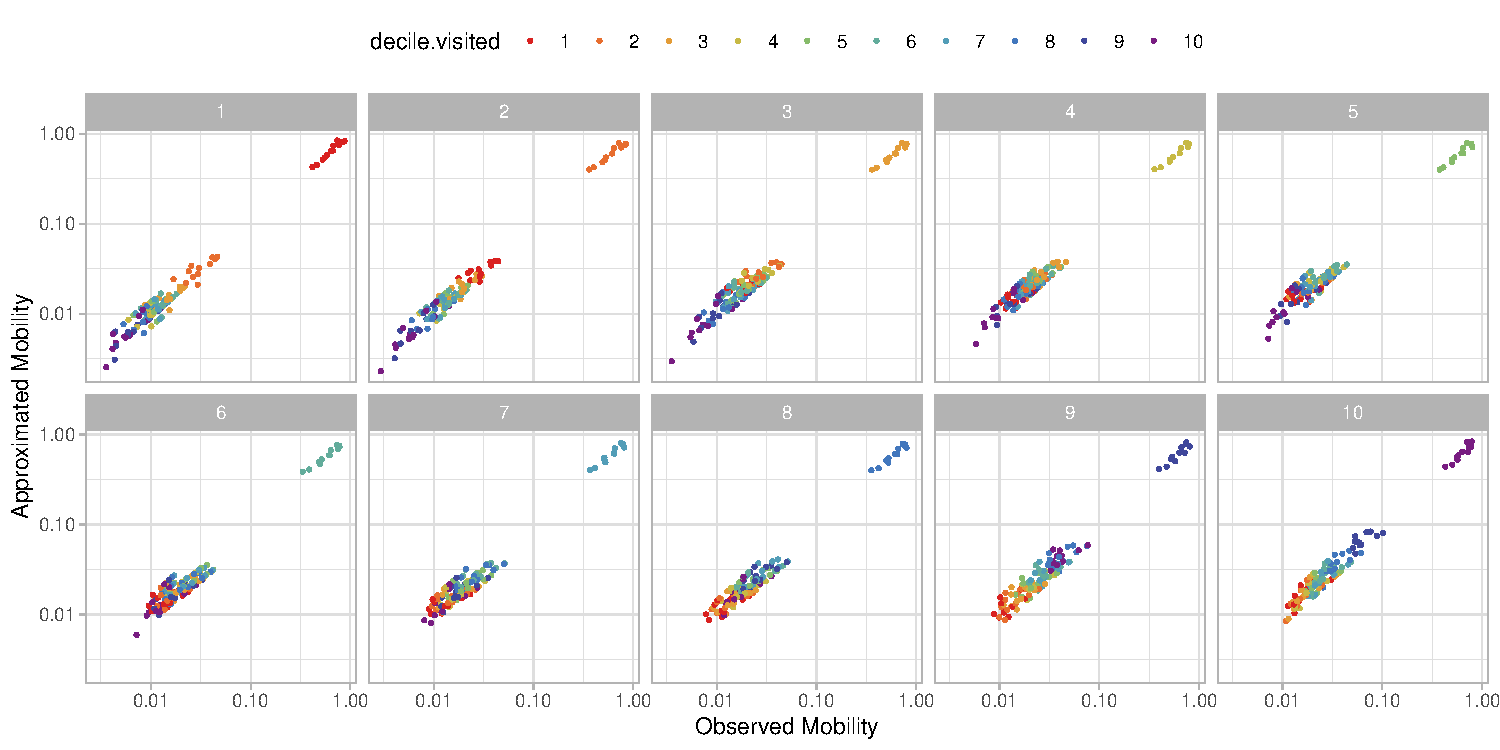
\includegraphics[height=\maxheight]{B-vs-Ba}
\end{frame}
% ------------------------------------------------------------------------------
\begin{frame}{Mobility Matrix \only<2>{(log scale)}}
  \centering
  \only<1>{\centering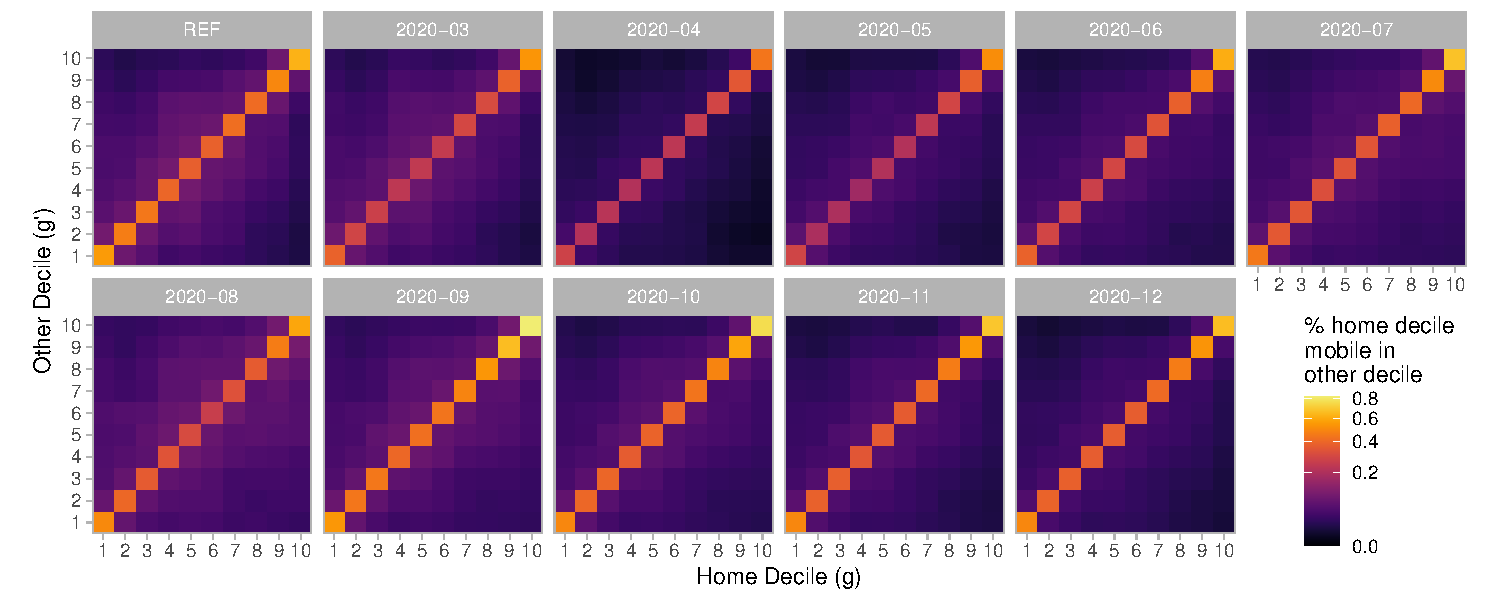
\includegraphics[height=\maxheight]{Bggt}}%
  \only<2>{\centering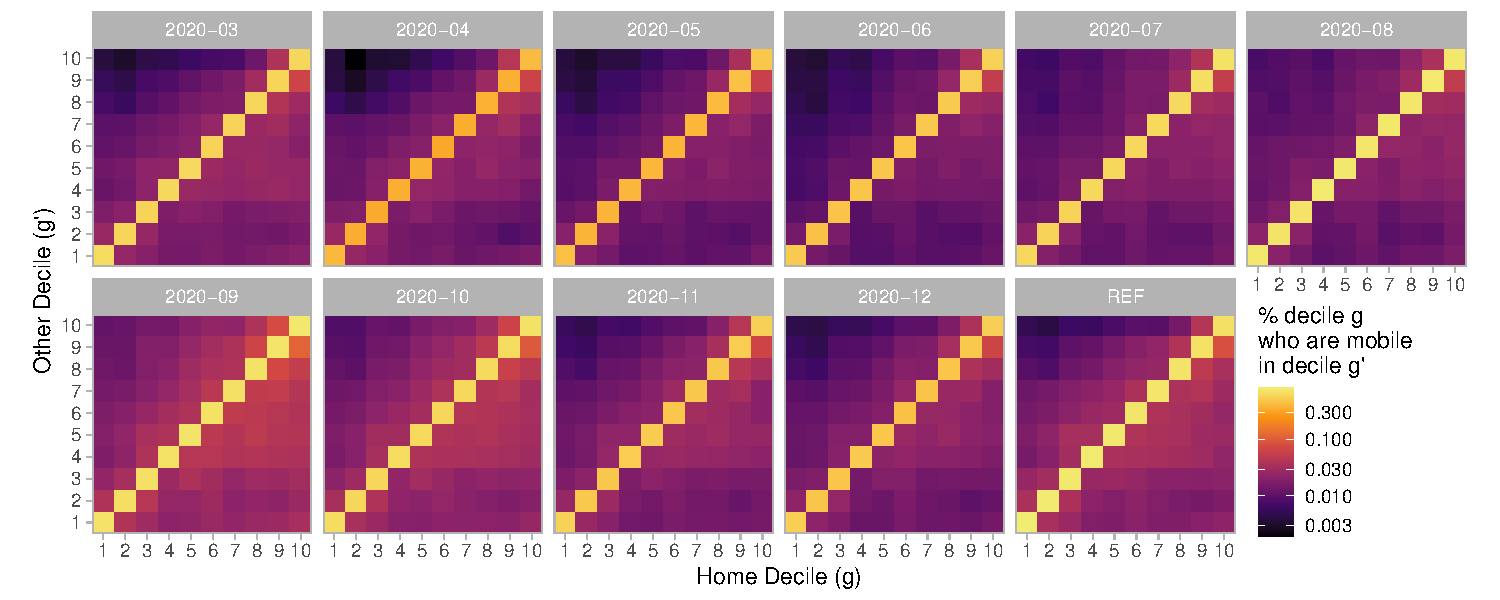
\includegraphics[height=\maxheight]{Bggt-log}}
\end{frame}
% ------------------------------------------------------------------------------
\begin{frame}{Mobility Matrix: Comment}
  \begin{itemize}
    \item Inter-FSA mobility mainly with similar deciles
          ($B^c_{gg'}$ clustered near diagonal)\smallpar
    \item Most \% time away from household within Home FSA
          ($\phi \approx 0.7$)\smallpar
    \item Lowest incidence deciles ($g = 9,10$):\smallpar
    \begin{itemize}
      \item Least mobility reduction (largest $R^{\rho}_{g}$)\smallpar
      \item Most time outside Home FSA (smallest $R^{\phi}_{g}$)\smallpar
    \end{itemize}
  \end{itemize}
\end{frame}
% ==============================================================================
\section{Age Mixing}
% ------------------------------------------------------------------------------
\begin{frame}{Prem et al (2021): \textsc{polymod} projected onto 177 countries, incl. Canada}
  \centerline{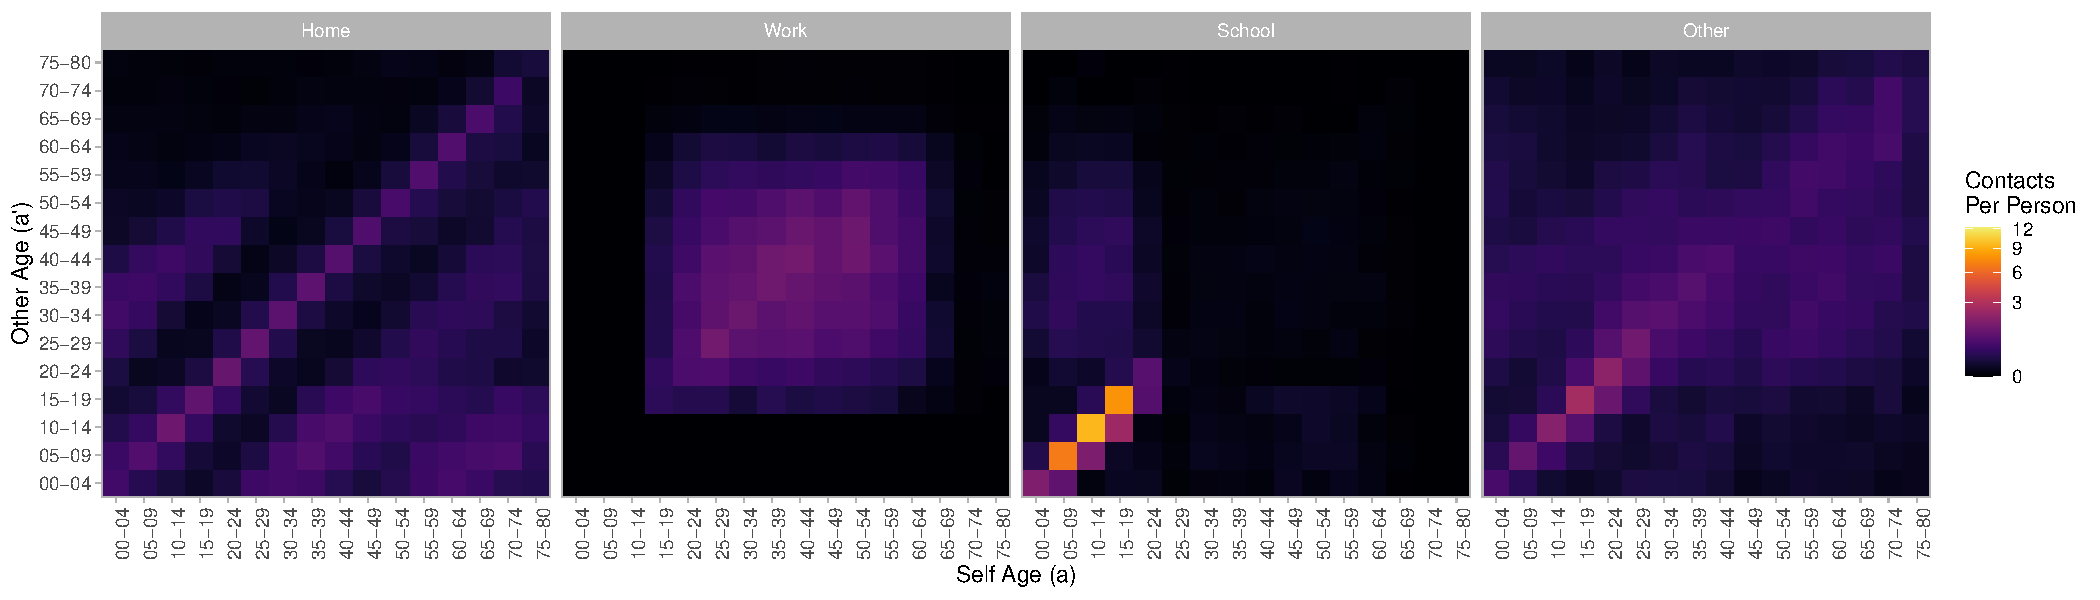
\includegraphics[width=\linewidth]{C4AAy0}}
  \bigpar
  Open source: \texttt{github.com/kieshaprem/synthetic-contact-matrices}
\end{frame}
% ------------------------------------------------------------------------------
\begin{frame}{Age Mixing, Challenge 1: contacts don't ``balance''}
  \paragraph{Solution}
  \bigpar
  \begin{tabular}{ll}
    \textbf{Un-weight} by Prem 2021 age group sizes $P_a$: &
    $C^u_{aa'y} = C_{aa'y} \frac{\bar{P}}{P_{a'}}$
    \\[\eqtabsep]
    \textbf{Enforce Symmetry} by averaging with transpose: &
    $C^{ub}_{aa'y} = \frac{1}{2}\left[C^u_{aa'y} + {C^u_{aa'y}}^T\right]$
  \end{tabular}
\end{frame}
% ------------------------------------------------------------------------------
\begin{frame}{Age Mixing, Challenge 1: balancing contacts}
  \centering
  \only<1>{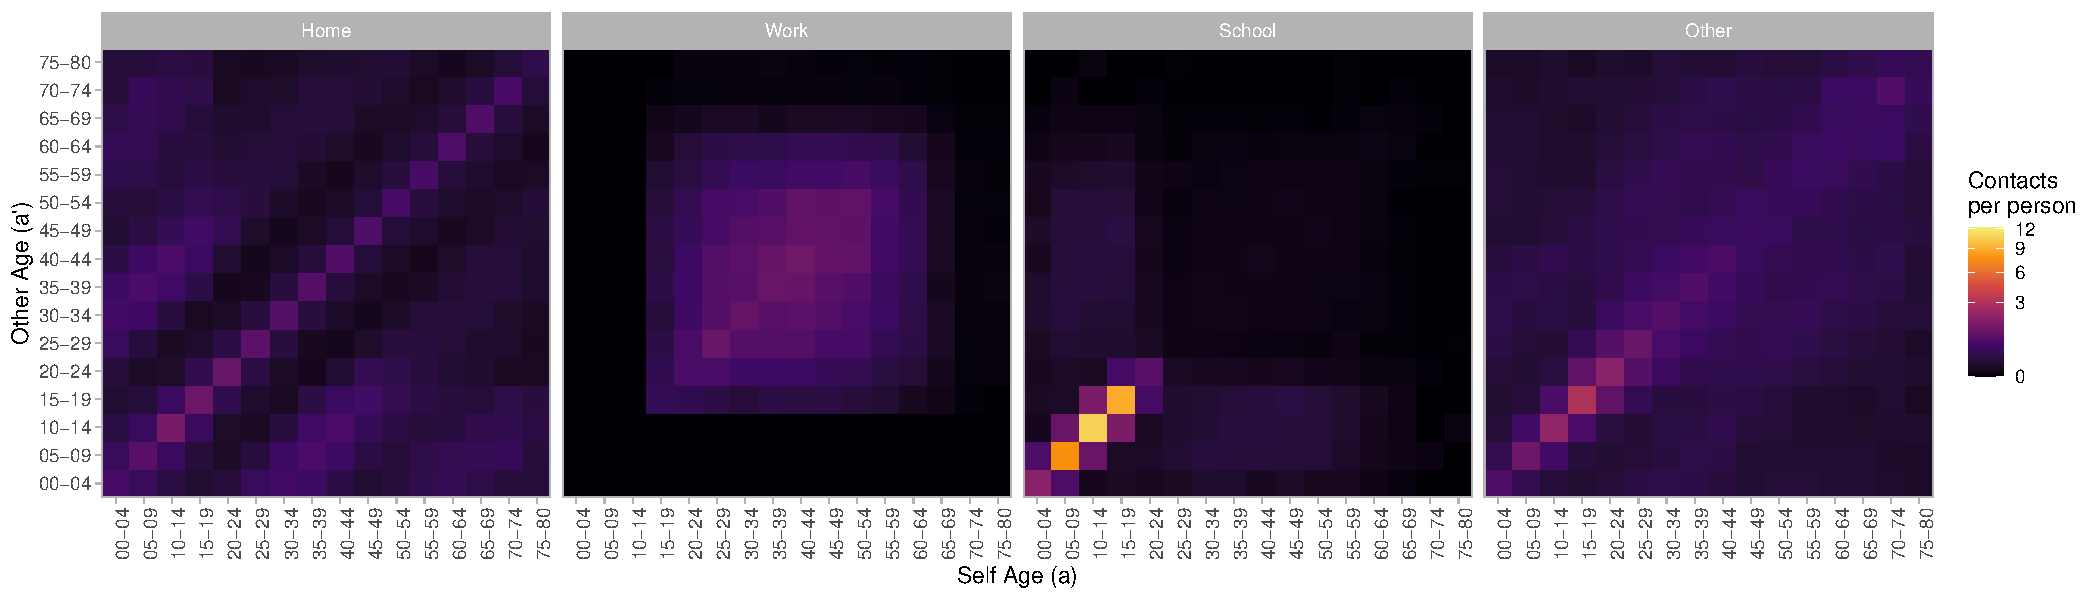
\includegraphics[width=\linewidth]{C4AAy}}%
  \only<2>{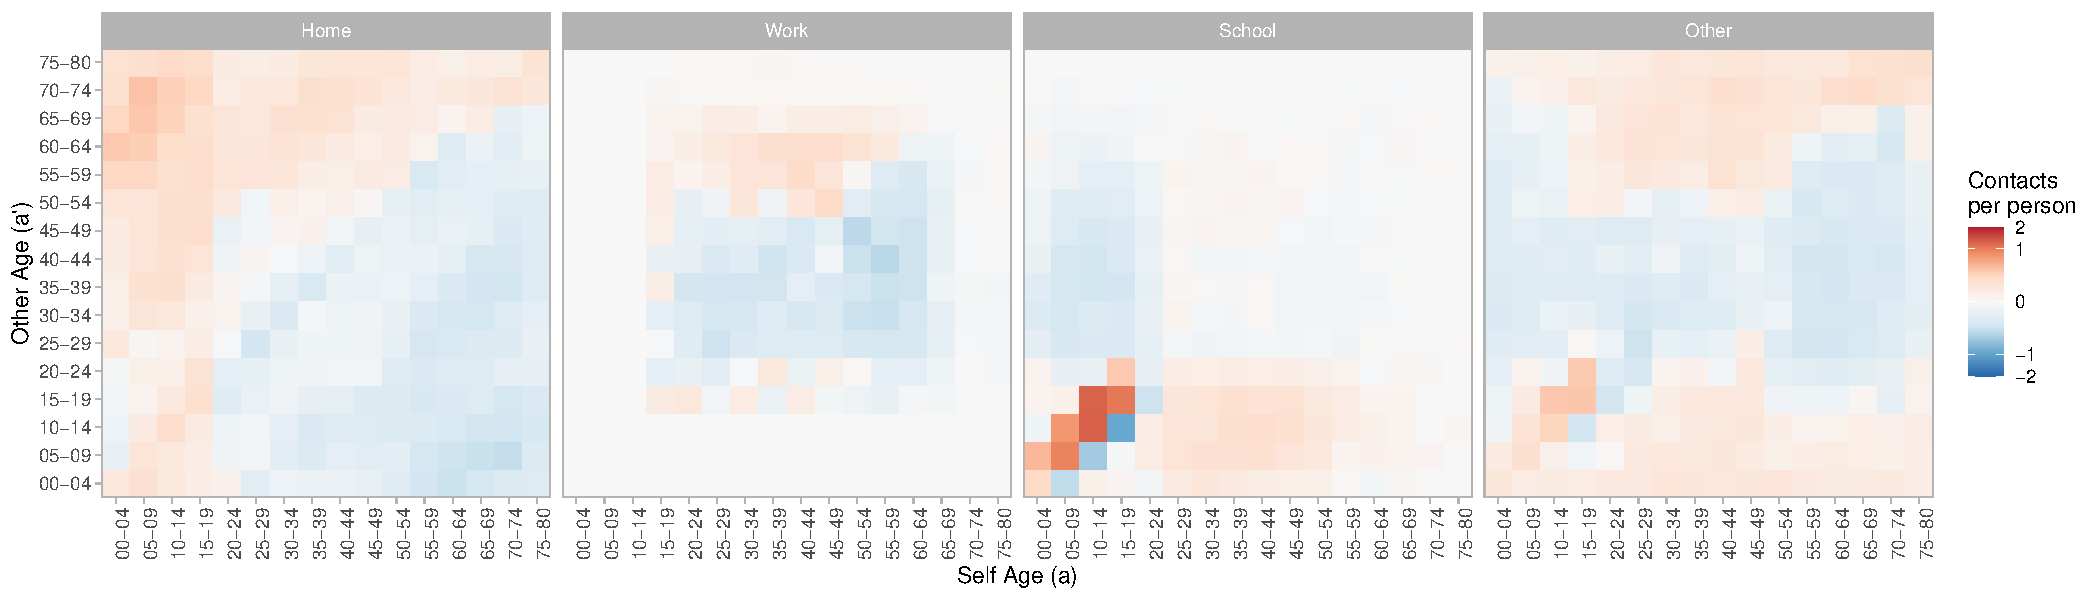
\includegraphics[width=\linewidth]{C4AAy-d02}}
\end{frame}
% ------------------------------------------------------------------------------
\begin{frame}{Age Mixing, Challenge 2: age stratifications don't align}
  \paragraph{Solution}
  \bigpar
  \begin{tabular}{ll}
    \textbf{Linear Upsample} from 5-year $\rightarrow$ 1-year age groups & \\[\eqtabsep]
    \textbf{Diagonally Pad} edges for 80+ age groups & \\[\eqtabsep]
    \textbf{Aggregate} 1-year $\rightarrow$ target age groups & \\[\eqtabsep]
  \end{tabular}
\end{frame}
% ------------------------------------------------------------------------------
\begin{frame}{Age Mixing, Challenge 2: re-stratify}
  \centering
  \only<1>{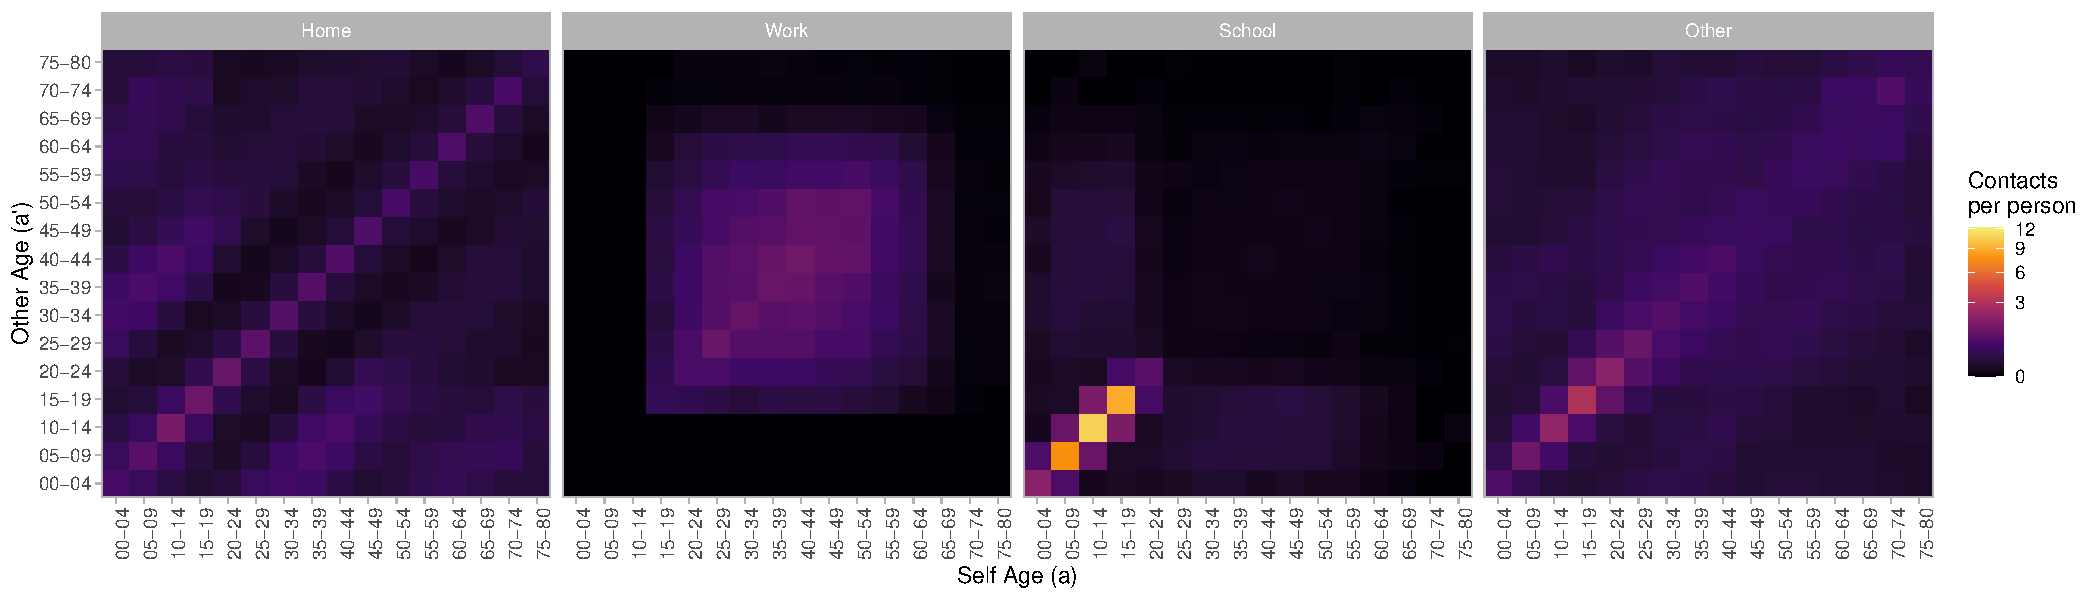
\includegraphics[width=\linewidth]{C4AAy}}%
  \only<2>{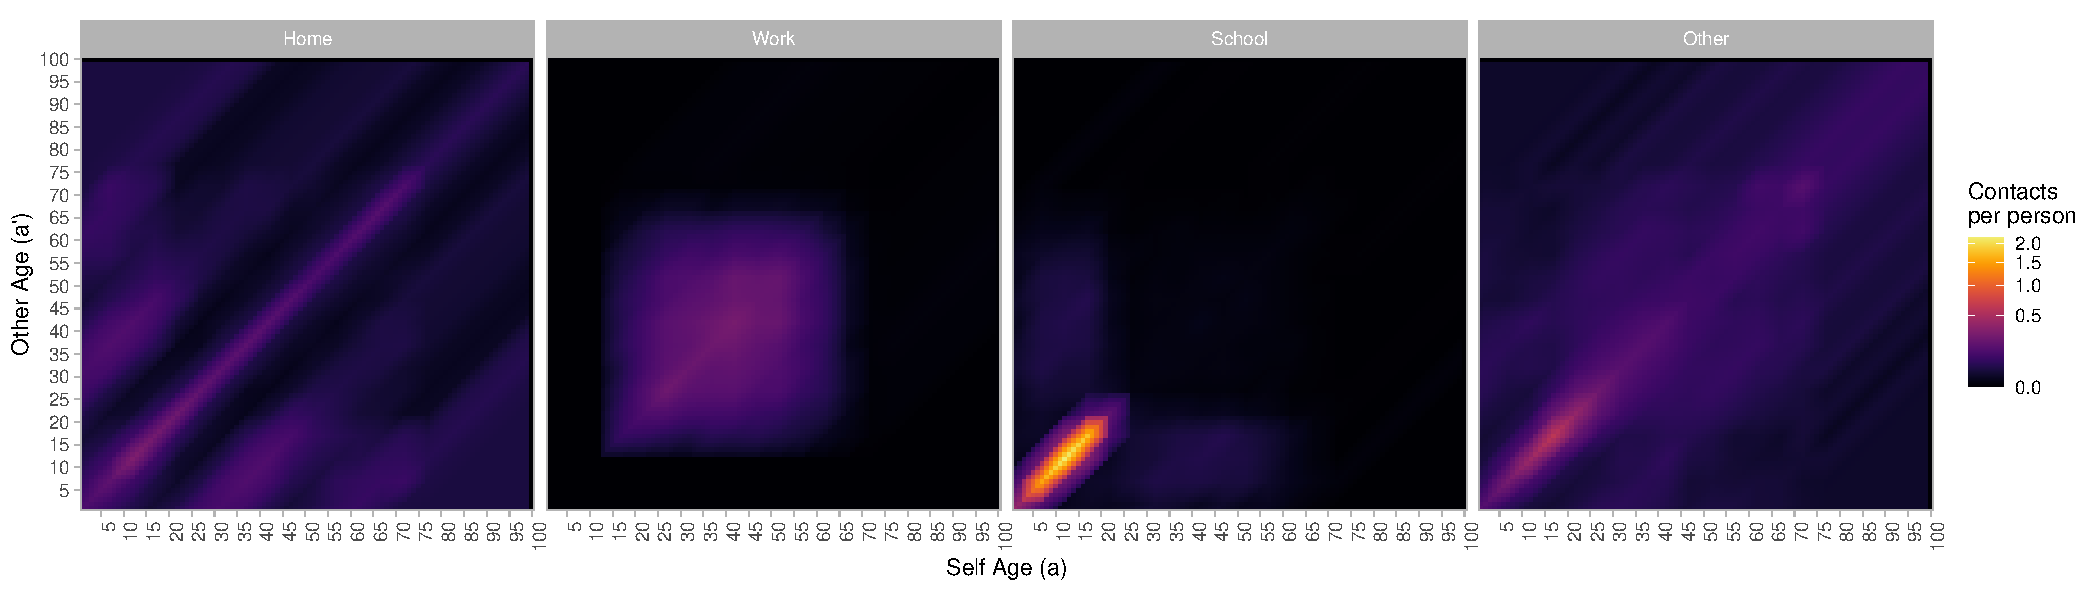
\includegraphics[width=\linewidth]{C411y}}%
  \only<3>{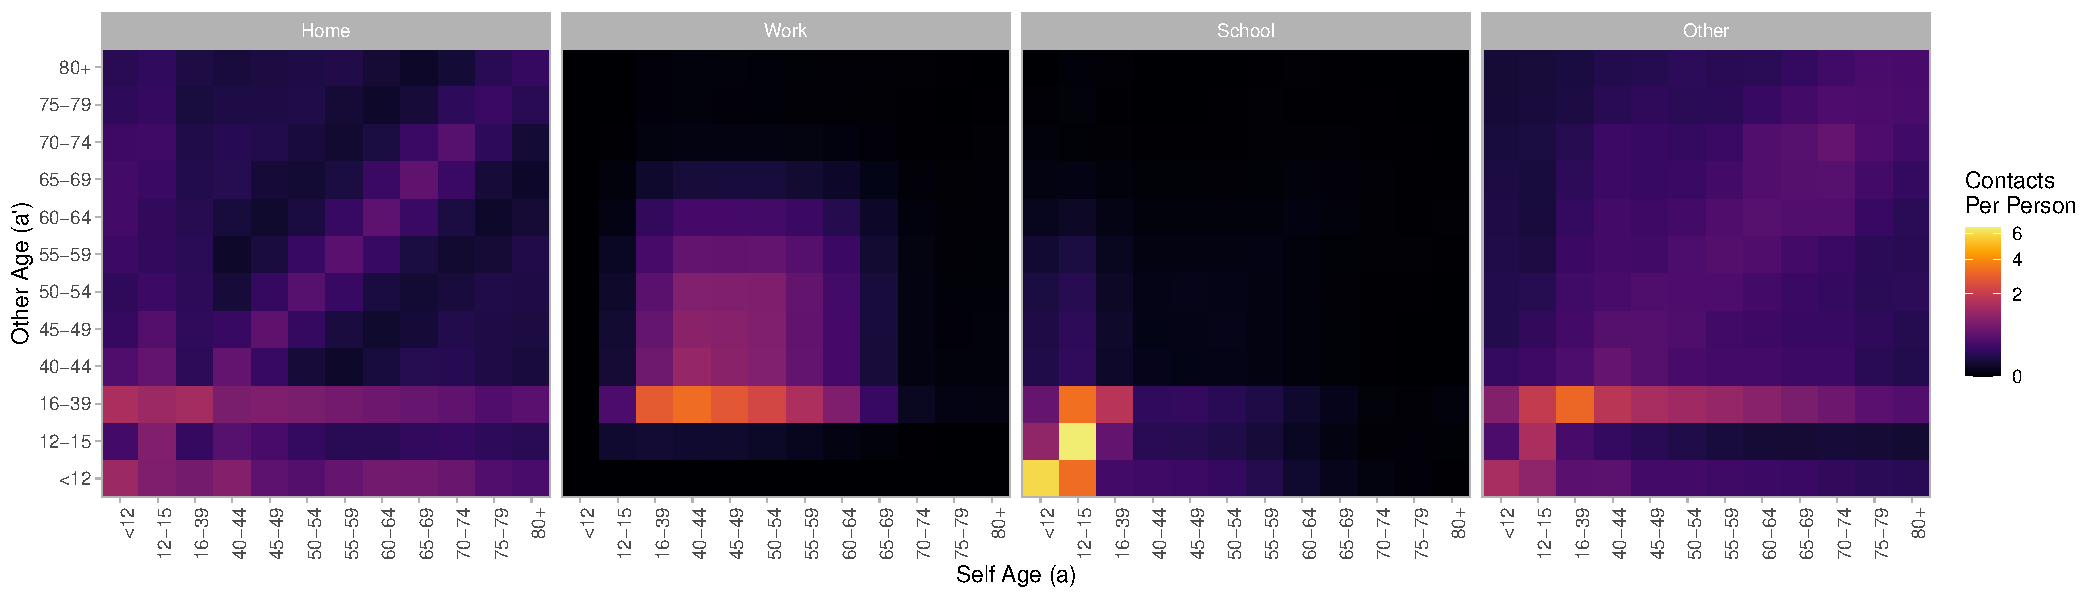
\includegraphics[width=\linewidth]{C4aay}}%
\end{frame}
% ------------------------------------------------------------------------------
\begin{frame}{Age Mixing: total contacts by age group}
  \centering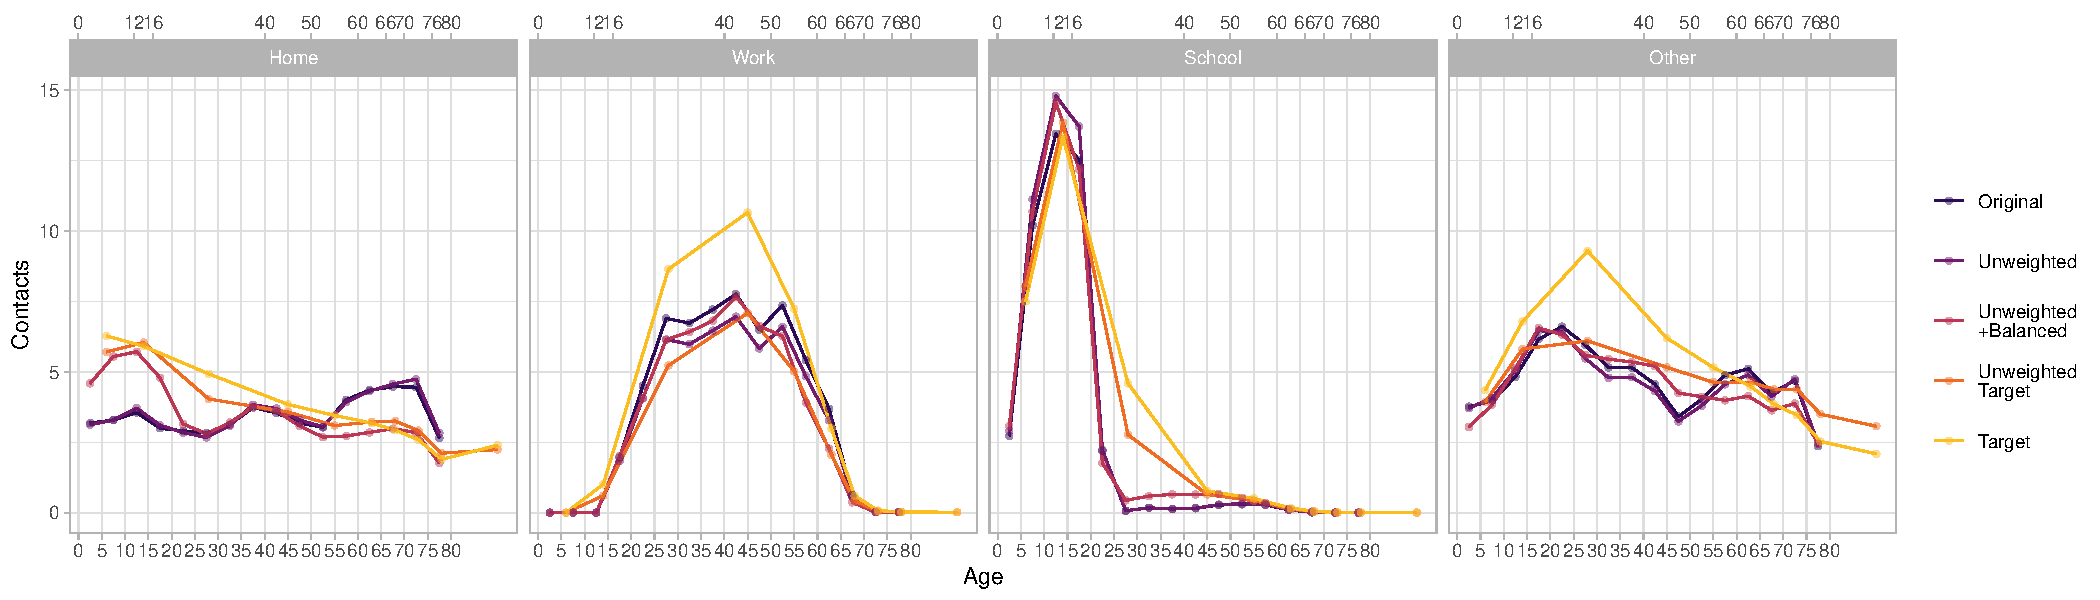
\includegraphics[width=\linewidth]{C4ay}
\end{frame}
% ------------------------------------------------------------------------------
\begin{frame}{Mobility Matrix: Comment}
  \begin{itemize}
    \item Adapting to different demographic structure: like Arregui et al. (2018)\smallpar
    \item New contributions: re-sampling strategy \& diagonal padding\smallpar
    \item Horizontal streaks are expected: due to unequal age groups
  \end{itemize}
\end{frame}
% ==============================================================================
\section{Combined Mixing}
% ------------------------------------------------------------------------------
\begin{frame}{Mixing Pools: Definitions}
  \begin{minipage}{0.5\linewidth}
    \pause
    \textbf{Home Pools}: contacts with Home FSA only\\\null\quad$(h_y) \delta_{gg'}$
    \bigpar
    \pause
    \textbf{Travel Pools}: contacts with other mobile
    \medpar
    \begin{itemize}
      \pause
      \item \textbf{Mobile at Home}: within Home FSA\\\quad$(1-h_y) B_{g = g'}$
      \medpar
      \pause
      \item \textbf{Mobile Away}: outside Home FSA\\\quad$(1-h_y) B_{g \ne g'}$
    \end{itemize}
  \end{minipage}%
  \begin{minipage}{0.5\linewidth}
    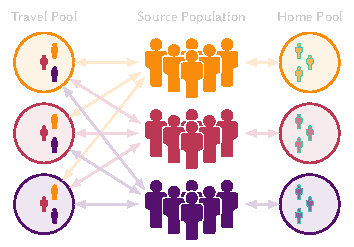
\includegraphics[width=\linewidth]{pools-half-home}
  \end{minipage}
\end{frame}
% ------------------------------------------------------------------------------
\begin{frame}{Mixing Pools as microcosms: Travel pool $g^*$}
  \begin{tabular}{ll}
    \textbf{Who} is here: &
    $P^{\,g^*}_{gay} = (1-h_y) B_{gg^*} P_{ga}$
    \\[\eqtabsep]
    \textbf{Proportionate} mixing of groups: &
    $X^{\,g^*r}_{gag'a'y} = \displaystyle\frac
      {P^{\,g^*}_{gay} \,\otimes\, P^{\,g^*}_{g'a'y}}
      {\sum_{g'a'} P^{\,g^*}_{g'a'y}}$
    \\[\eqtabsep]
    \textbf{Contacts by age} applied on top: &
    $X^{\,g^*}_{gag'a'y} = X^{\,g^*r}_{gag'a'y} C^{ub}_{aa'y} w^{-1}_{a'}$
  \end{tabular}
  \bigpar\bigpar
  Home pool $g^*$: same, except $(1-h_y) B_{gg^*} \rightarrow (h_y)\delta_{gg^*}$
  \vskip-\eqtabsep
\end{frame}
% ------------------------------------------------------------------------------
\begin{frame}[fragile]{Total contacts across mixing pools}
  \begin{minipage}{0.45\linewidth}
    \paragraph{Total \# Contacts}
    \begin{equation*}
      X_{gag'a'y} =
      \ulabel{X^h_{gag'a'y}}{home pool} +
      \ulabel{\textstyle\sum_{g^*} X^{\,g^*}_{gag'a'y}}{travel pools}
    \end{equation*}
    \paragraph{\# Contacts per Person}
    \begin{equation*}
      C_{gag'a'y} = \displaystyle\frac{X_{gag'a'y}}{P_{ga}}
    \end{equation*}
  \end{minipage}\hfill\Large$\bm{\rightarrow}$\hfill%
  \begin{minipage}{0.45\linewidth}\footnotesize
      \verb| g, g',  a, a',         y,   t,     C|
      \verb| 1,  1, <4, <4, household, Jan, 0.592|
      \verb| 1,  1, <4, <4, household, Feb, 0.541|
      \verb| 1,  1, <4, <4, household, Mar, 0.604|
      \verb|...|
  \end{minipage}
\end{frame}
% ------------------------------------------------------------------------------
\begin{frame}{Contacts per person: age vs age ($a,a'$)}
  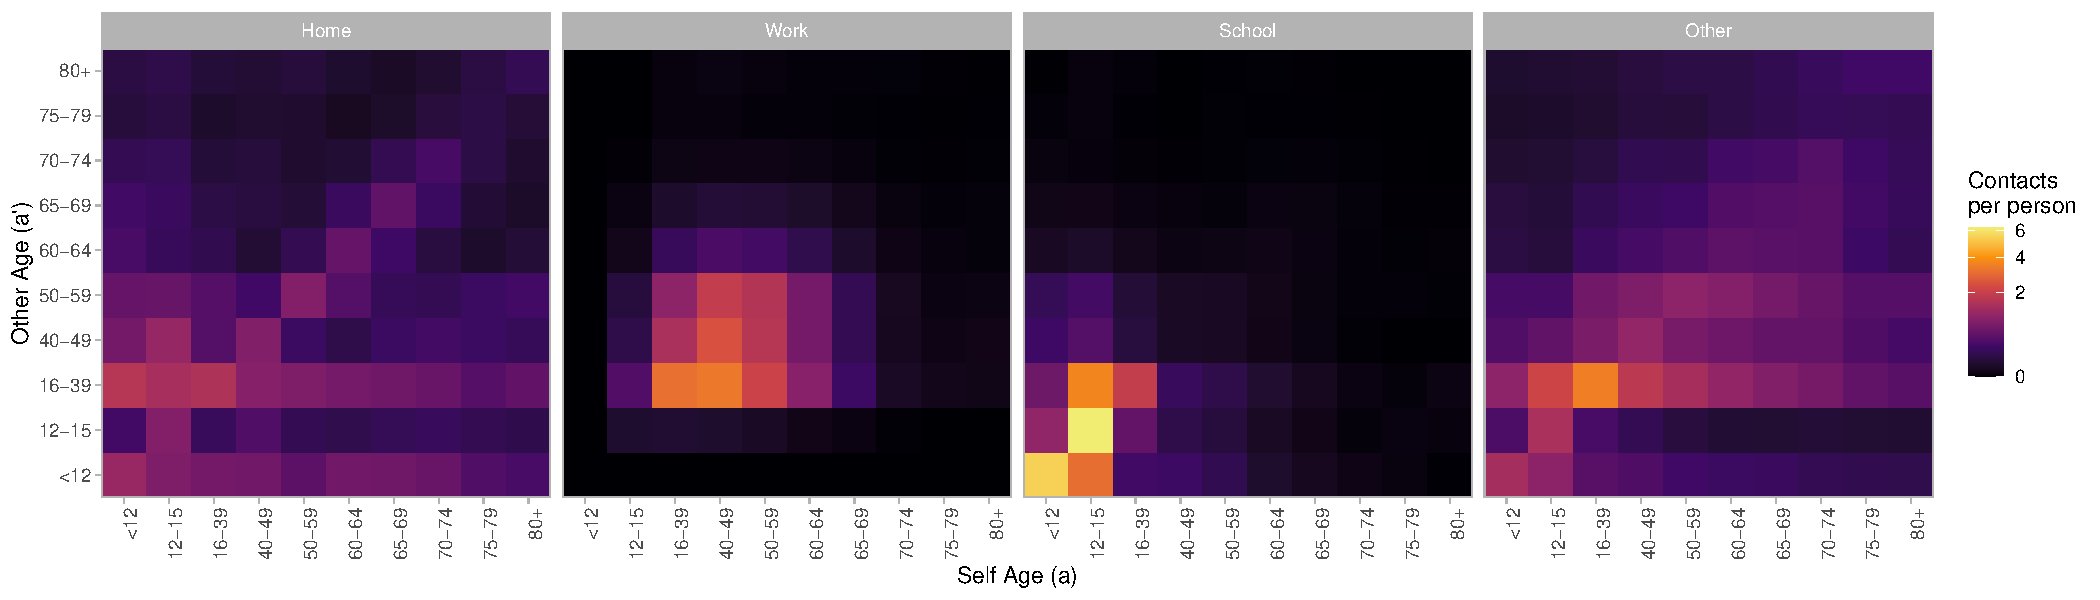
\includegraphics[width=\linewidth]{CX4aay}
\end{frame}
% ------------------------------------------------------------------------------
\begin{frame}{Contacts per person: decile vs decile ($g,g'$)}
  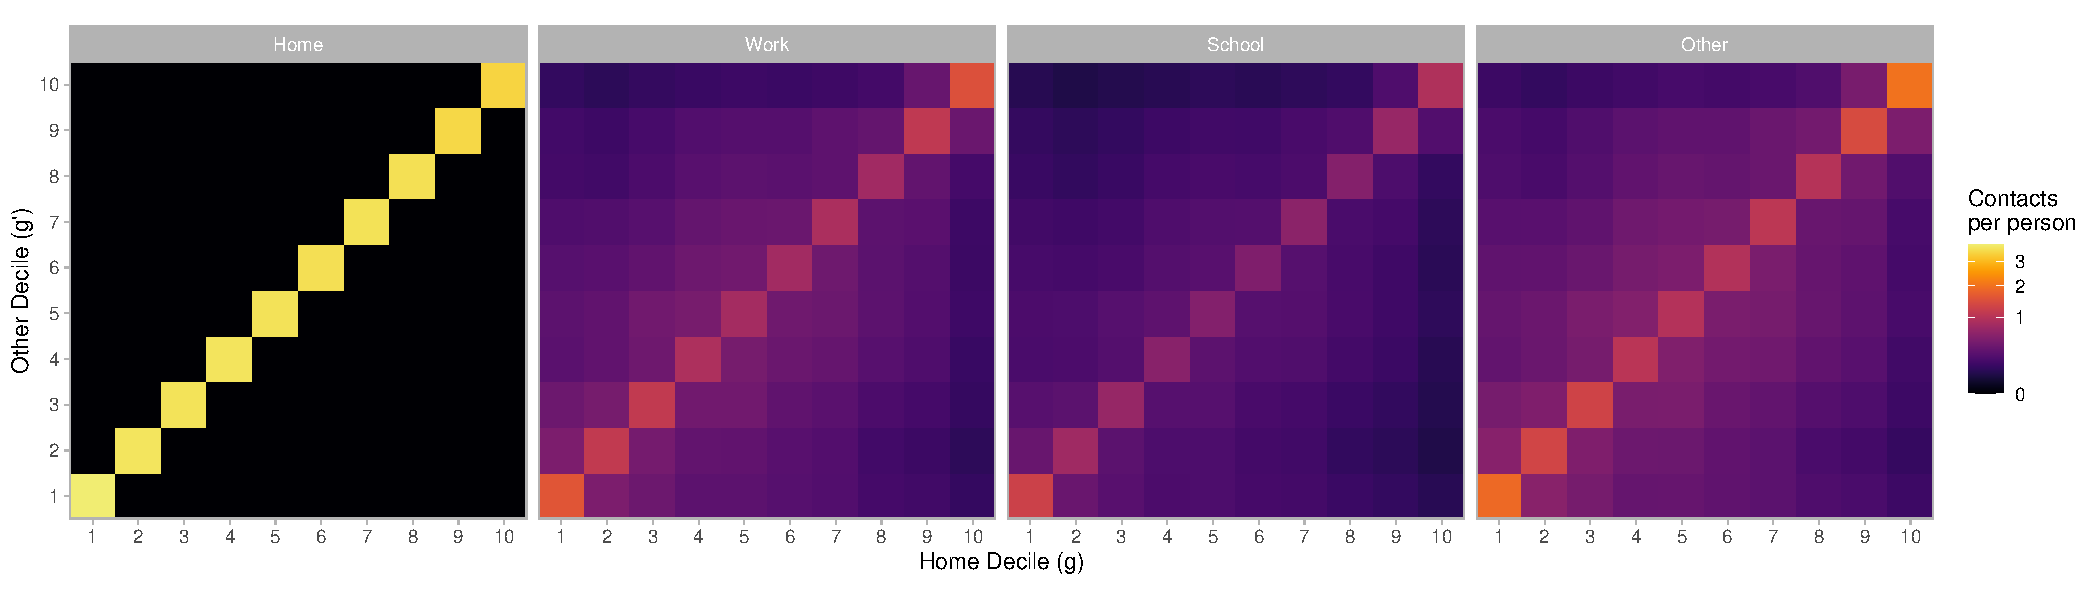
\includegraphics[width=\linewidth]{CX4ggy}
\end{frame}
% ------------------------------------------------------------------------------
\begin{frame}{Contacts per person: all types ($y$)}
  \centering
  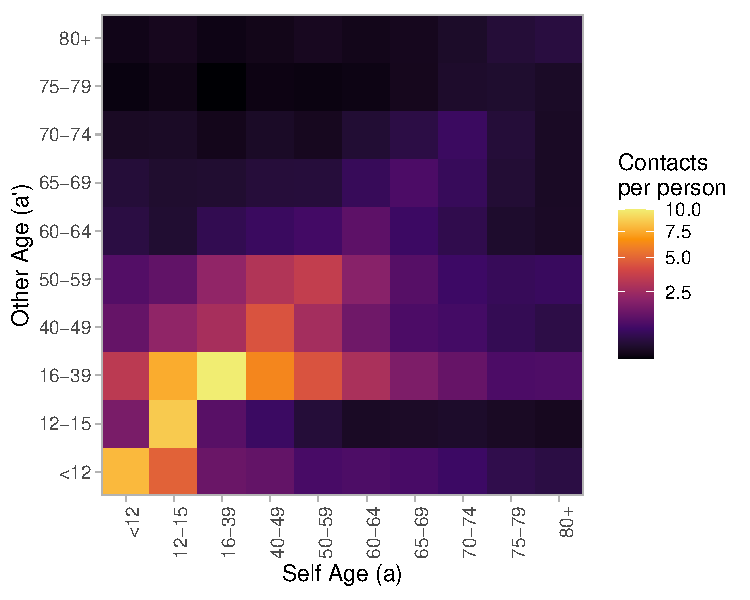
\includegraphics[width=.45\linewidth]{CXaay}
  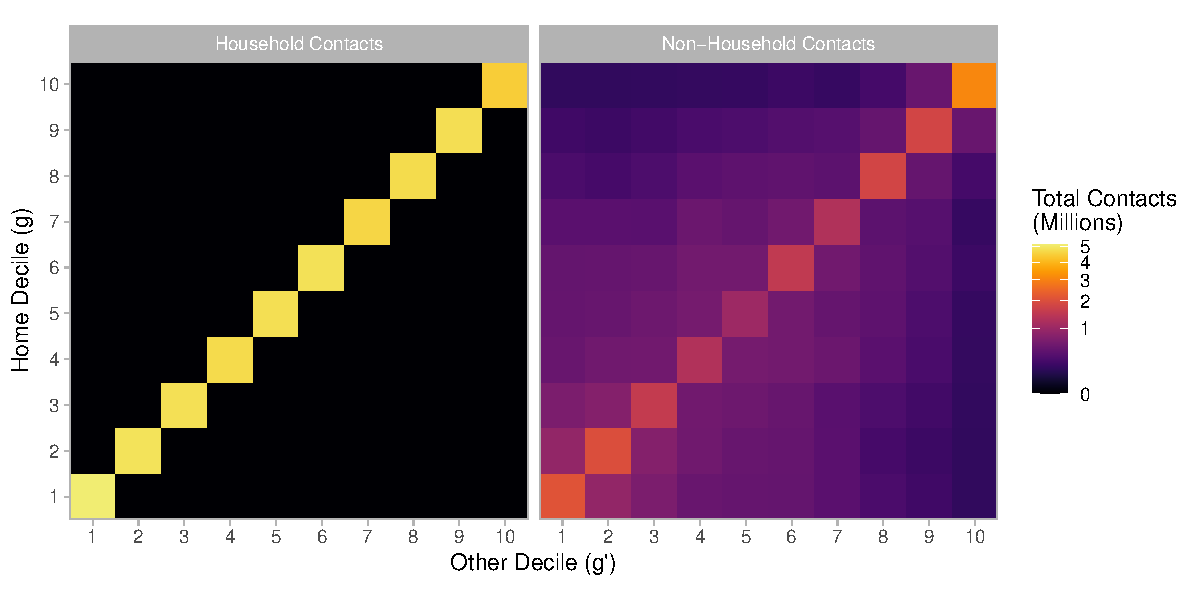
\includegraphics[width=.45\linewidth]{CXggy}
\end{frame}
% ------------------------------------------------------------------------------
\begin{frame}{Combined Mixing: Comment}
  \begin{itemize}
    \item Recurrent mobility approach: like Arenas et al. (2020)
    \item Recurrent mobility allows people from A \& B to mix in C\\
          $\rightarrow$ connectivity is greater than mobility would suggest
    \item New contributions: home vs travel pools, combined age mixing, balancing
  \end{itemize}
  \bigpar
  \paragraph{Next Steps}
  \begin{itemize}
    \item Validation of \# contacts with \covid surveys (BC Mix, \textsc{connect})
    \item Scaling contacts by decile for model fitting
  \end{itemize}
\end{frame}
% ------------------------------------------------------------------------------
\begin{frame}{Thanks}
  \centering
  Kristy~Yiu, Gary~Moloney, Linwei~Wang
  \vfill\hfill\hfill
  
\includegraphics[height=0.11\textheight]{nserc}\hfill
  
\includegraphics[height=0.10\textheight]{on}\hfill
  
\includegraphics[height=0.08\textheight]{smh}
  \hfill\hfill\null\bigpar\hfill\hfill
  
\includegraphics[height=0.12\textheight]{uoft}\hfill
  
\includegraphics[height=0.10\textheight]{map}
  \hfill\hfill\null
\end{frame}